
\section{Device Information APIs}

We have exposed only a focused subset of the Device Information APIs on our gateway, following the same selective approach we have applied to our other API families. This decision was driven by two key factors: the current capabilities provided by IT, and our focus on addressing the core needs of our primary use cases.

Our implementation specifically supports the following APIs: Device Reachability Status, Device Reachability Status Subscription, Device Roaming Status, and Device Roaming Status Subscription. Together, these services enable us to monitor the availability of devices and track their roaming behavior in real time, while also allowing clients to subscribe to status changes proactively. This allows dependent systems to adapt to changes in device connectivity or location with minimal latency and maximum efficiency.

\subsection{Device Reachability Status}

The Device Reachability Status API enables API consumers to query the current connectivity status of a device on the mobile network. The API provides real-time information on whether a device is reachable via SMS, data (mobile internet), or both, allowing businesses to make more informed communication and service management decisions based on the device’s availability.

The implementation uses 3GPP's Monitoring Event API with the monitoring type set to \Verb{UE_REACHABILITY} with a single report and finally it also sets the reachability type to both \Verb{DATA} and then \Verb{SMS}. This means that instead of sending a notification on the next check it is sent imediatly on the response from where we extract the most recent information about both SMS and Data reachability status.

\begin{figure}[H]
	\centerline{
		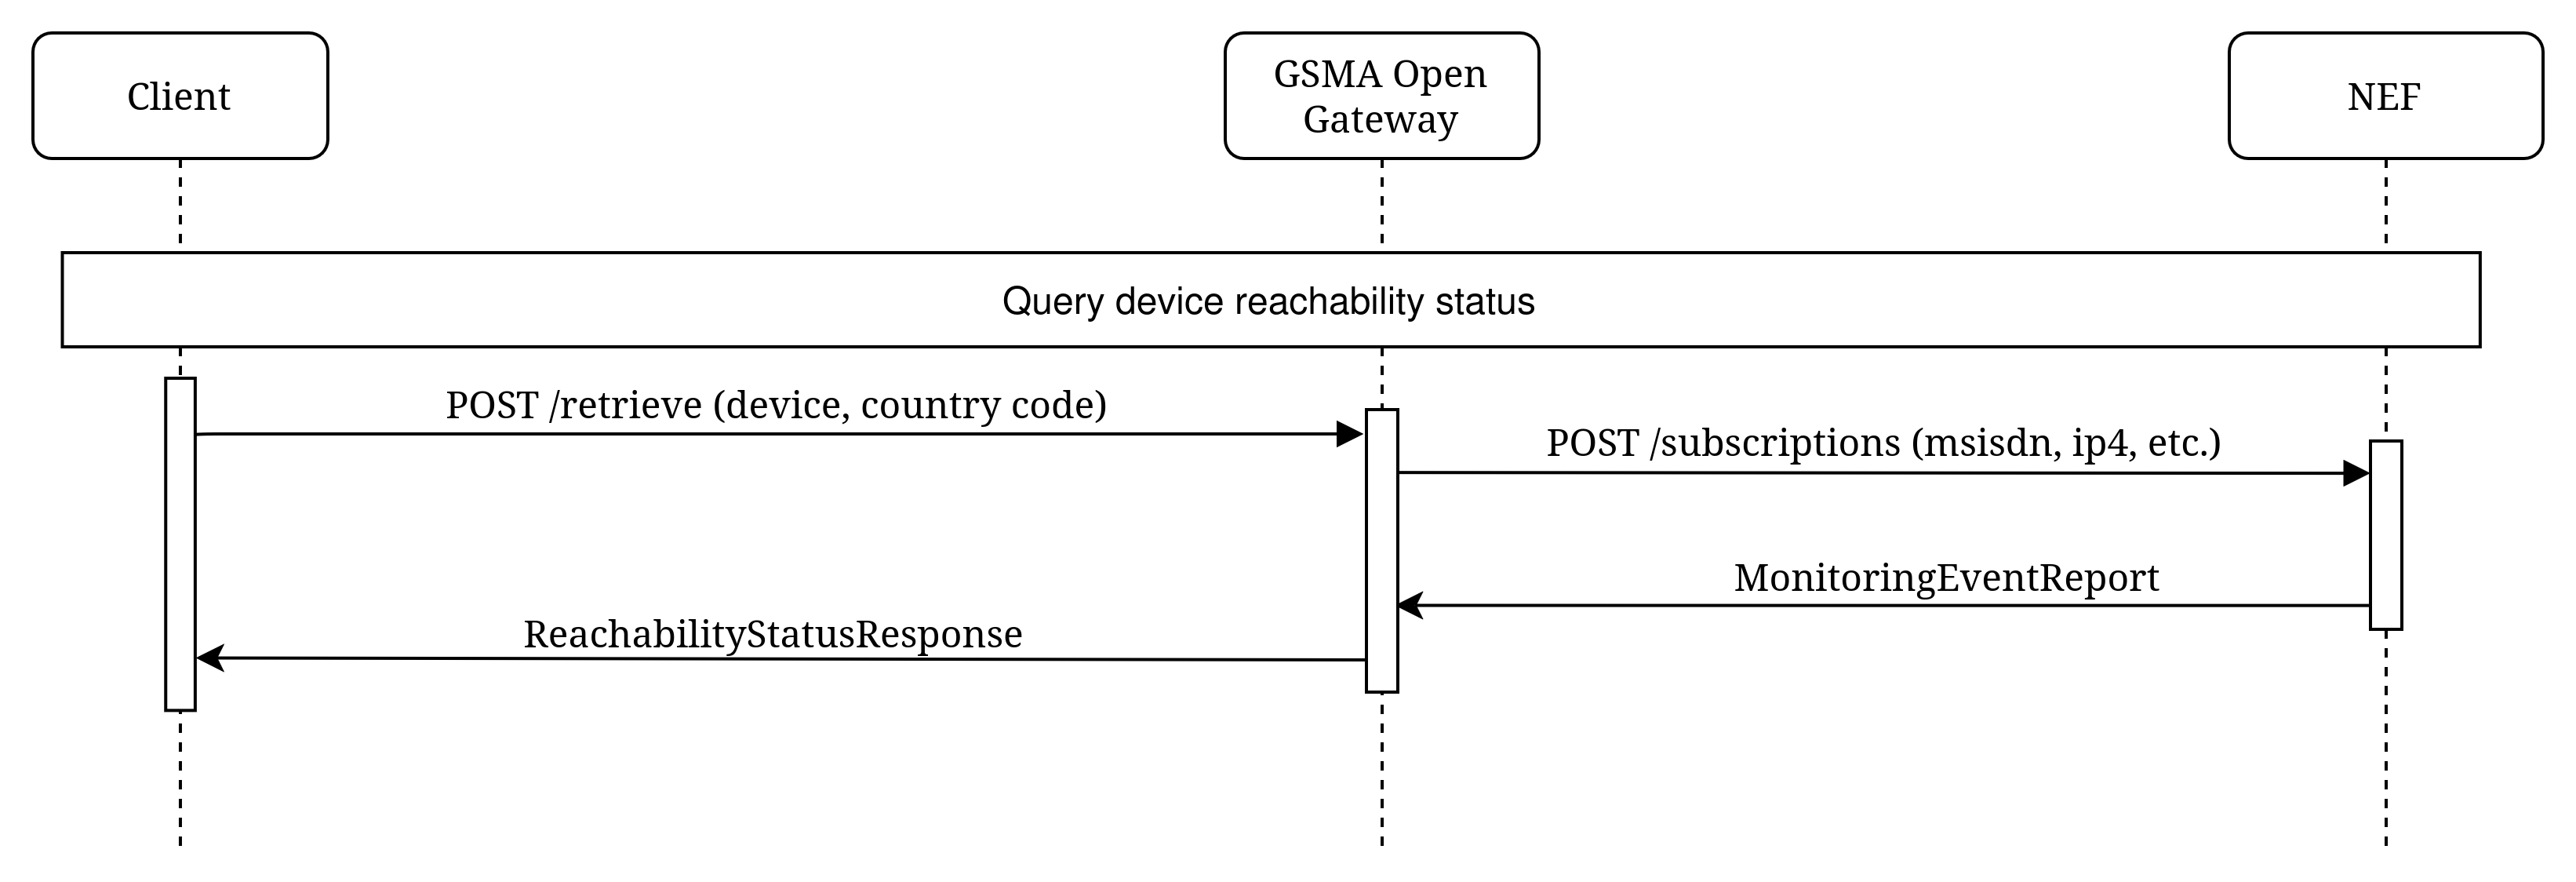
\includegraphics[width=10cm]{figs/reachability_status_sequence_diagram.png}
	}
	\caption{Device Reachability Status Sequence Diagram}
\end{figure}

\subsection{Device Reachability Status Subscription}

The Device Reachability Status Subscription API allows API consumers to subscribe to notifications about changes in a device’s connectivity status. Rather than performing repeated polling, clients can receive asynchronous updates when a device’s reachability over SMS, data, or both changes, enabling more efficient and timely service adjustments.

Our implementation leverages 3GPP's Monitoring Event API with the monitoring type set to \Verb{UE_REACHABILITY}. Unlike the one-time query used in the Device Reachability Status API, the subscription model registers an ongoing monitoring request, allowing the network to push updates whenever the reachability state changes. We configure the subscription to monitor either \Verb{DATA} or \Verb{SMS} reachability types, ensuring comprehensive coverage of the device's availability.

Furthermore, our implementation also supports retrieving the current status of all active subscriptions or querying specific subscription IDs for their details. Subscriptions can be cleanly removed via a dedicated delete operation, giving clients full control over the subscription lifecycle and resource management.

\begin{figure}[H]
	\centerline{
		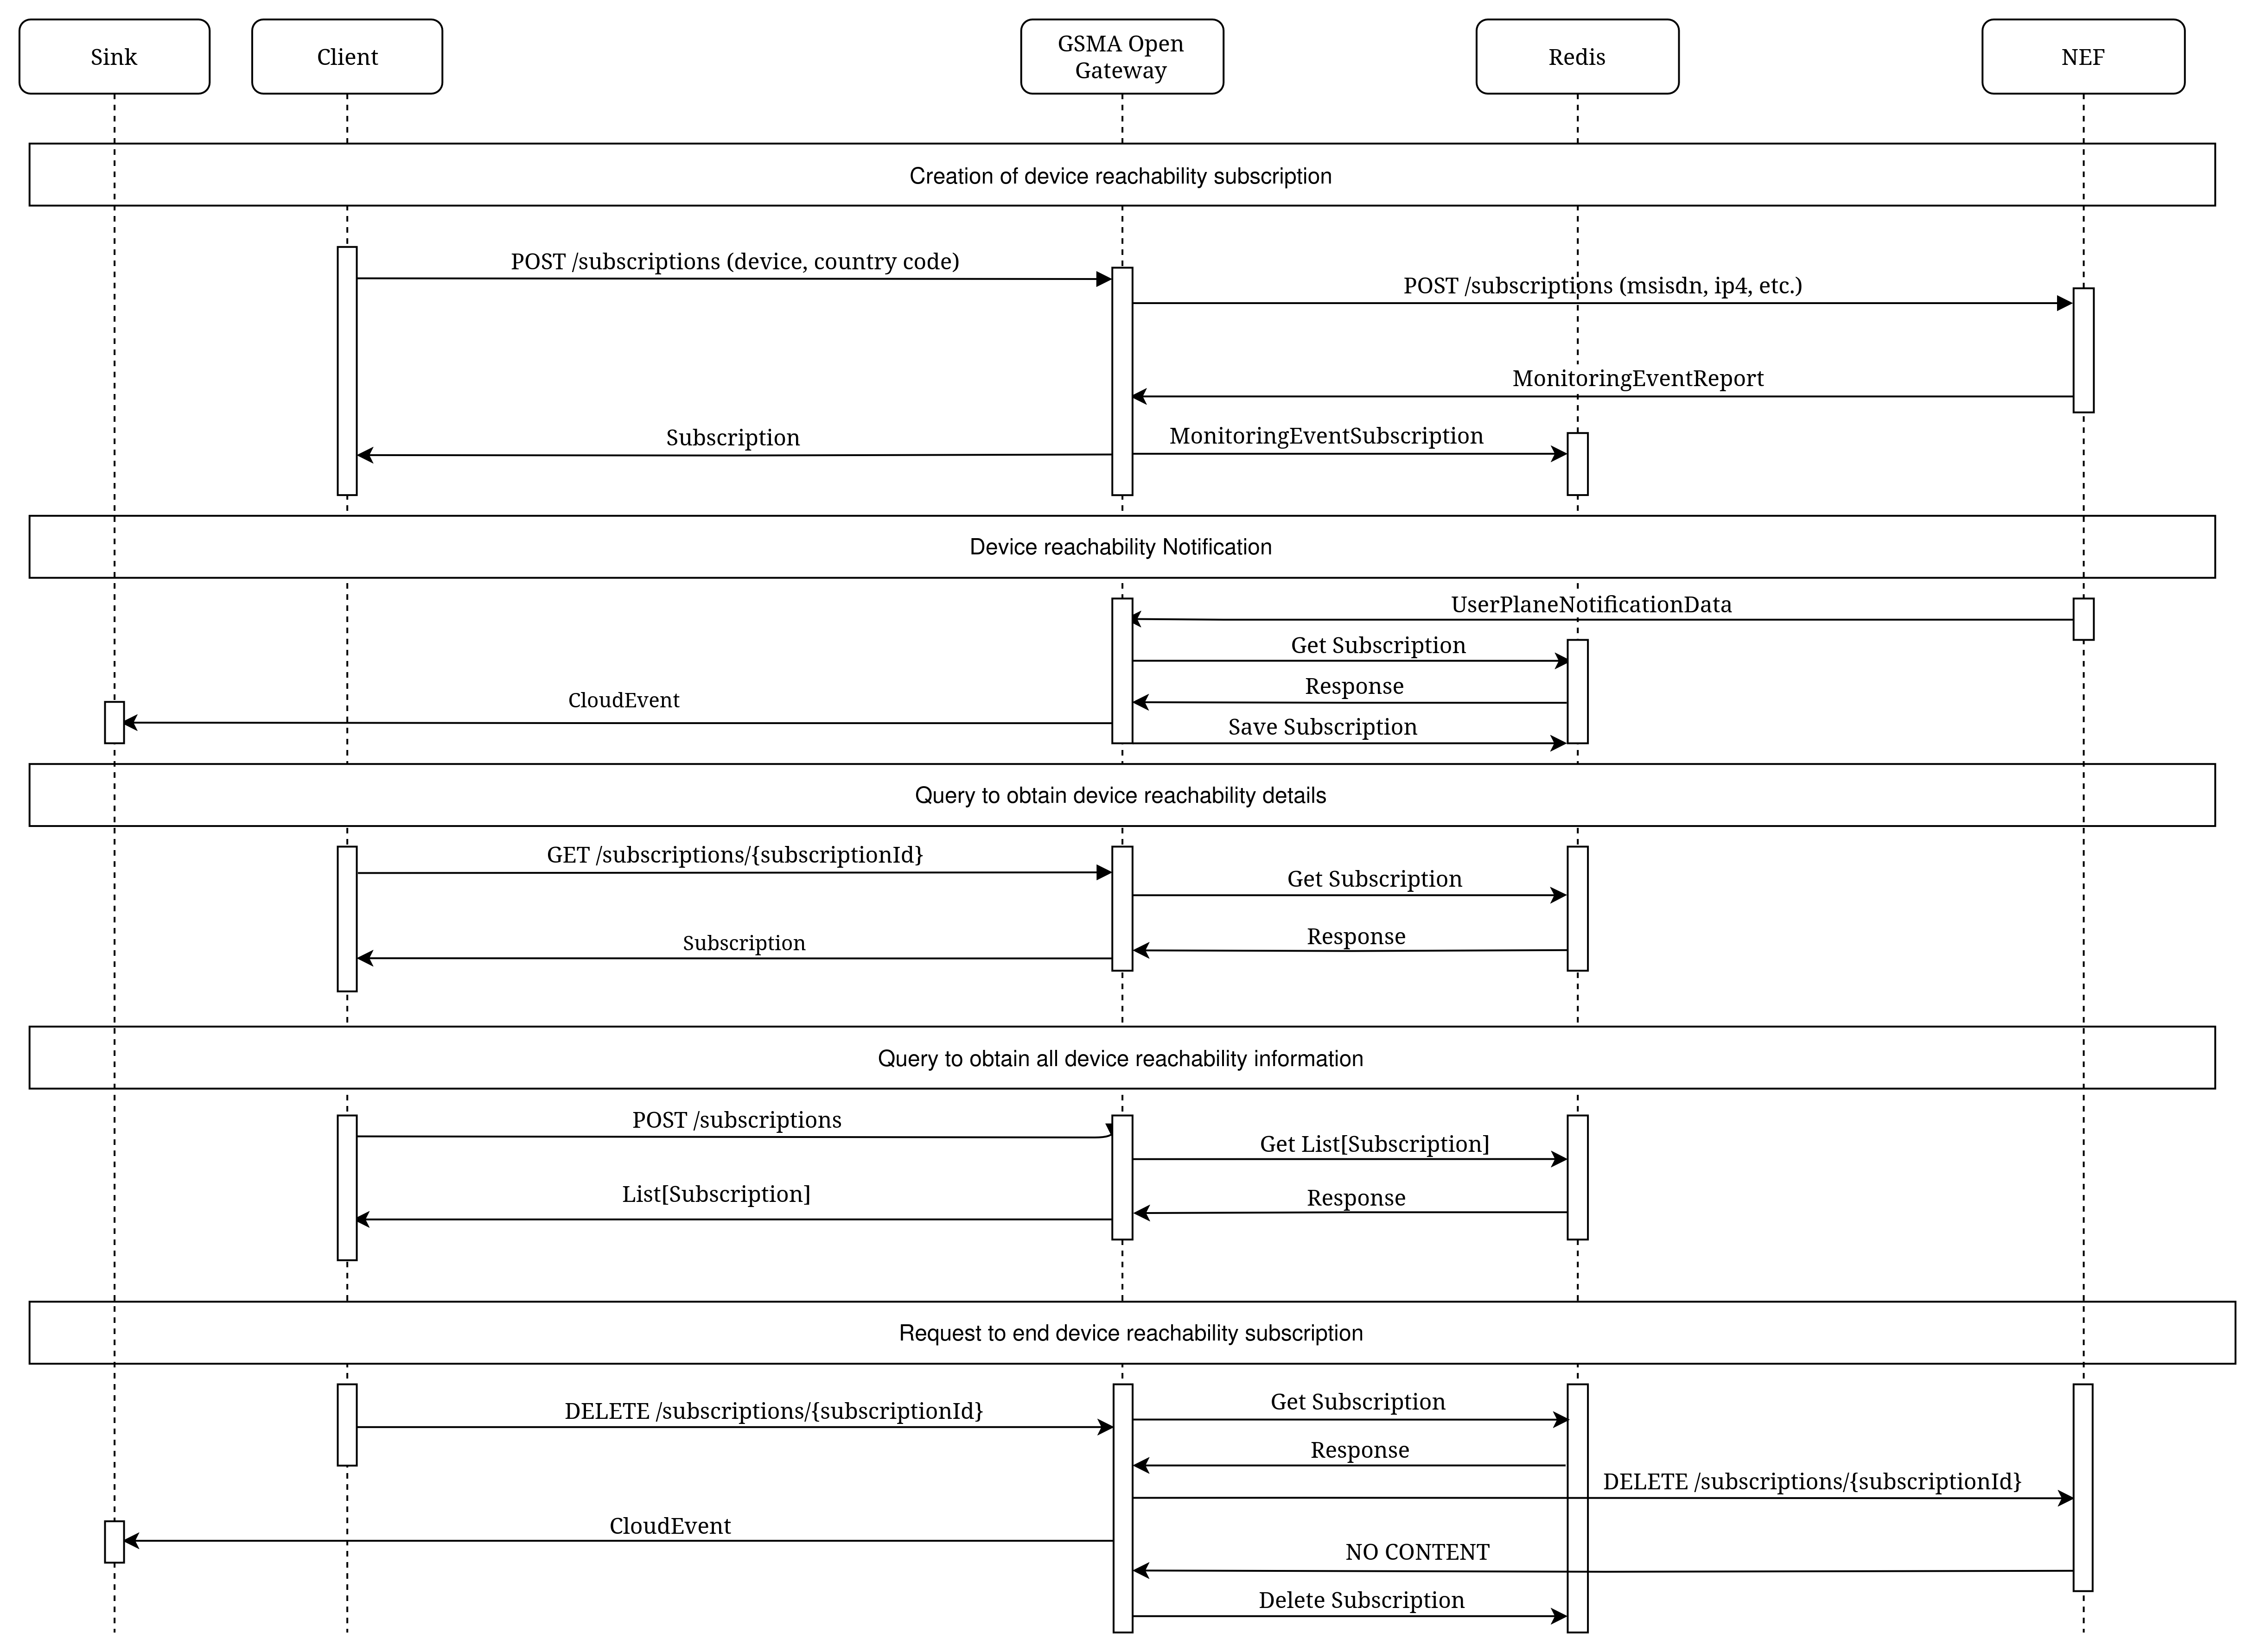
\includegraphics[width=15cm]{figs/reachability_status_sub_sequence_diagram.png}
	}
	\caption{Device Reachability Status Subscription Sequence Diagram}
\end{figure}

\subsection{Device Roaming Status}

The Device Roaming Status API enables developers to determine whether a device is roaming on a foreign mobile network and to identify the country in which it is currently located. This information supports fraud detection, regulatory compliance, and the enforcement of geo-based content restrictions.

Similar to the APIs described before, this uses 3GPP's Monitoring Event API, however the monitoring type is set to \Verb{ROAMING_STATUS} and with a single report. This means, like the Device Reachability Status API, the information is sent imediatly on the response from where we get the most recent information about the device's roaming status

\begin{figure}[H]
	\centerline{
		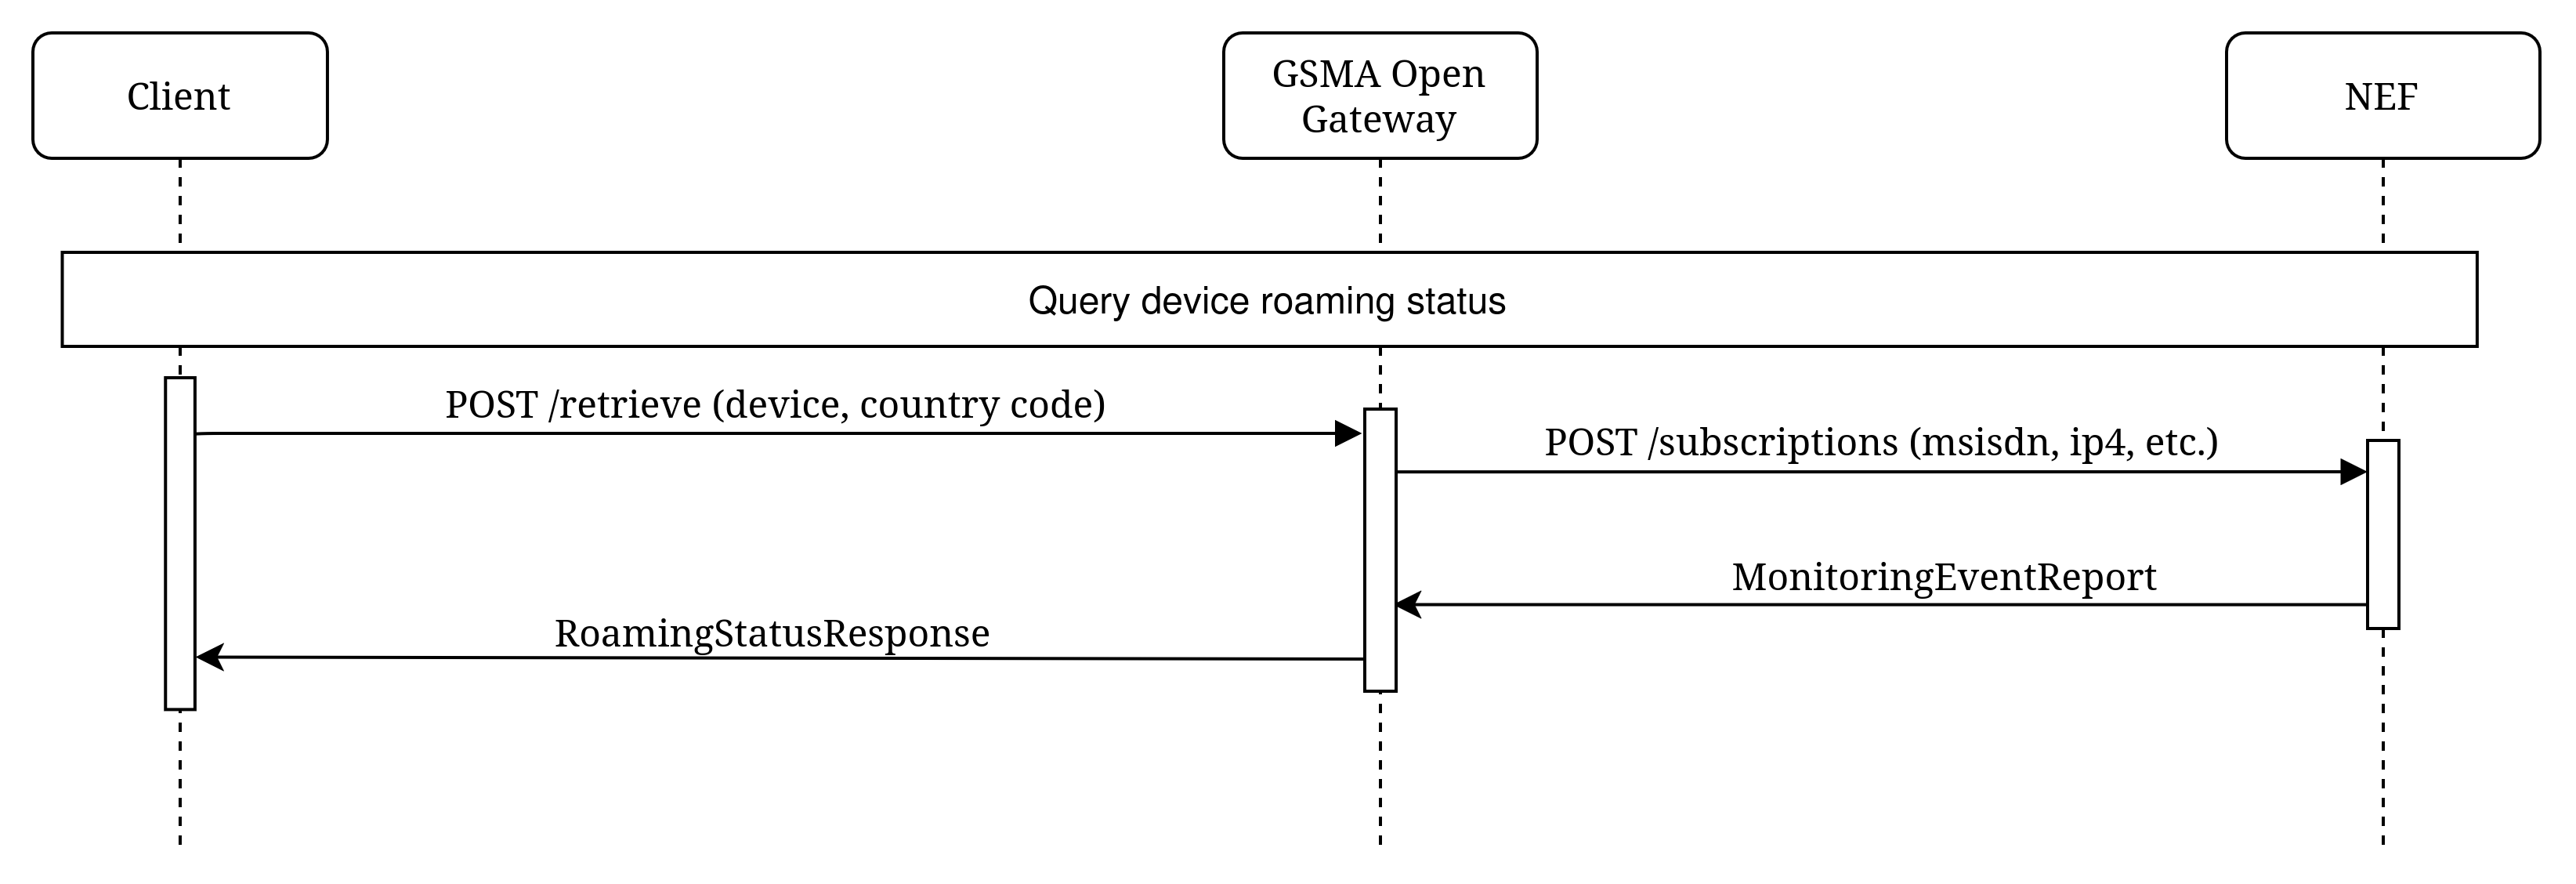
\includegraphics[width=10cm]{figs/roaming_sequence_diagram.png}
	}
	\caption{Device Roaming Status Sequence Diagram}
\end{figure}

\subsection{Device Roaming Status Subscription}

The Device Roaming Status Subscription API allows API consumers to receive asynchronous notifications whenever a device’s roaming status changes. This eliminates the need for repeated polling, enabling real-time awareness of roaming events that can be critical for fraud detection, regulatory enforcement, and geo-based service adjustments.

Our implementation is based on 3GPP's Monitoring Event API with the monitoring type, once more, set to \Verb{ROAMING_STATUS}. Unlike the one-time query used in the Device Roaming Status API, the subscription model establishes an ongoing monitoring request, allowing the network to proactively notify clients whenever the device's roaming state changes. Each update includes the roaming status, providing accurate and timely context for decision making.

In addition to subscribing, API consumers can retrieve a list of all active subscriptions or query specific subscription IDs to inspect their current configuration. Subscriptions can also be deleted as needed, allowing clients to efficiently manage resources and control subscription lifecycles.

\begin{figure}[H]
	\centerline{
		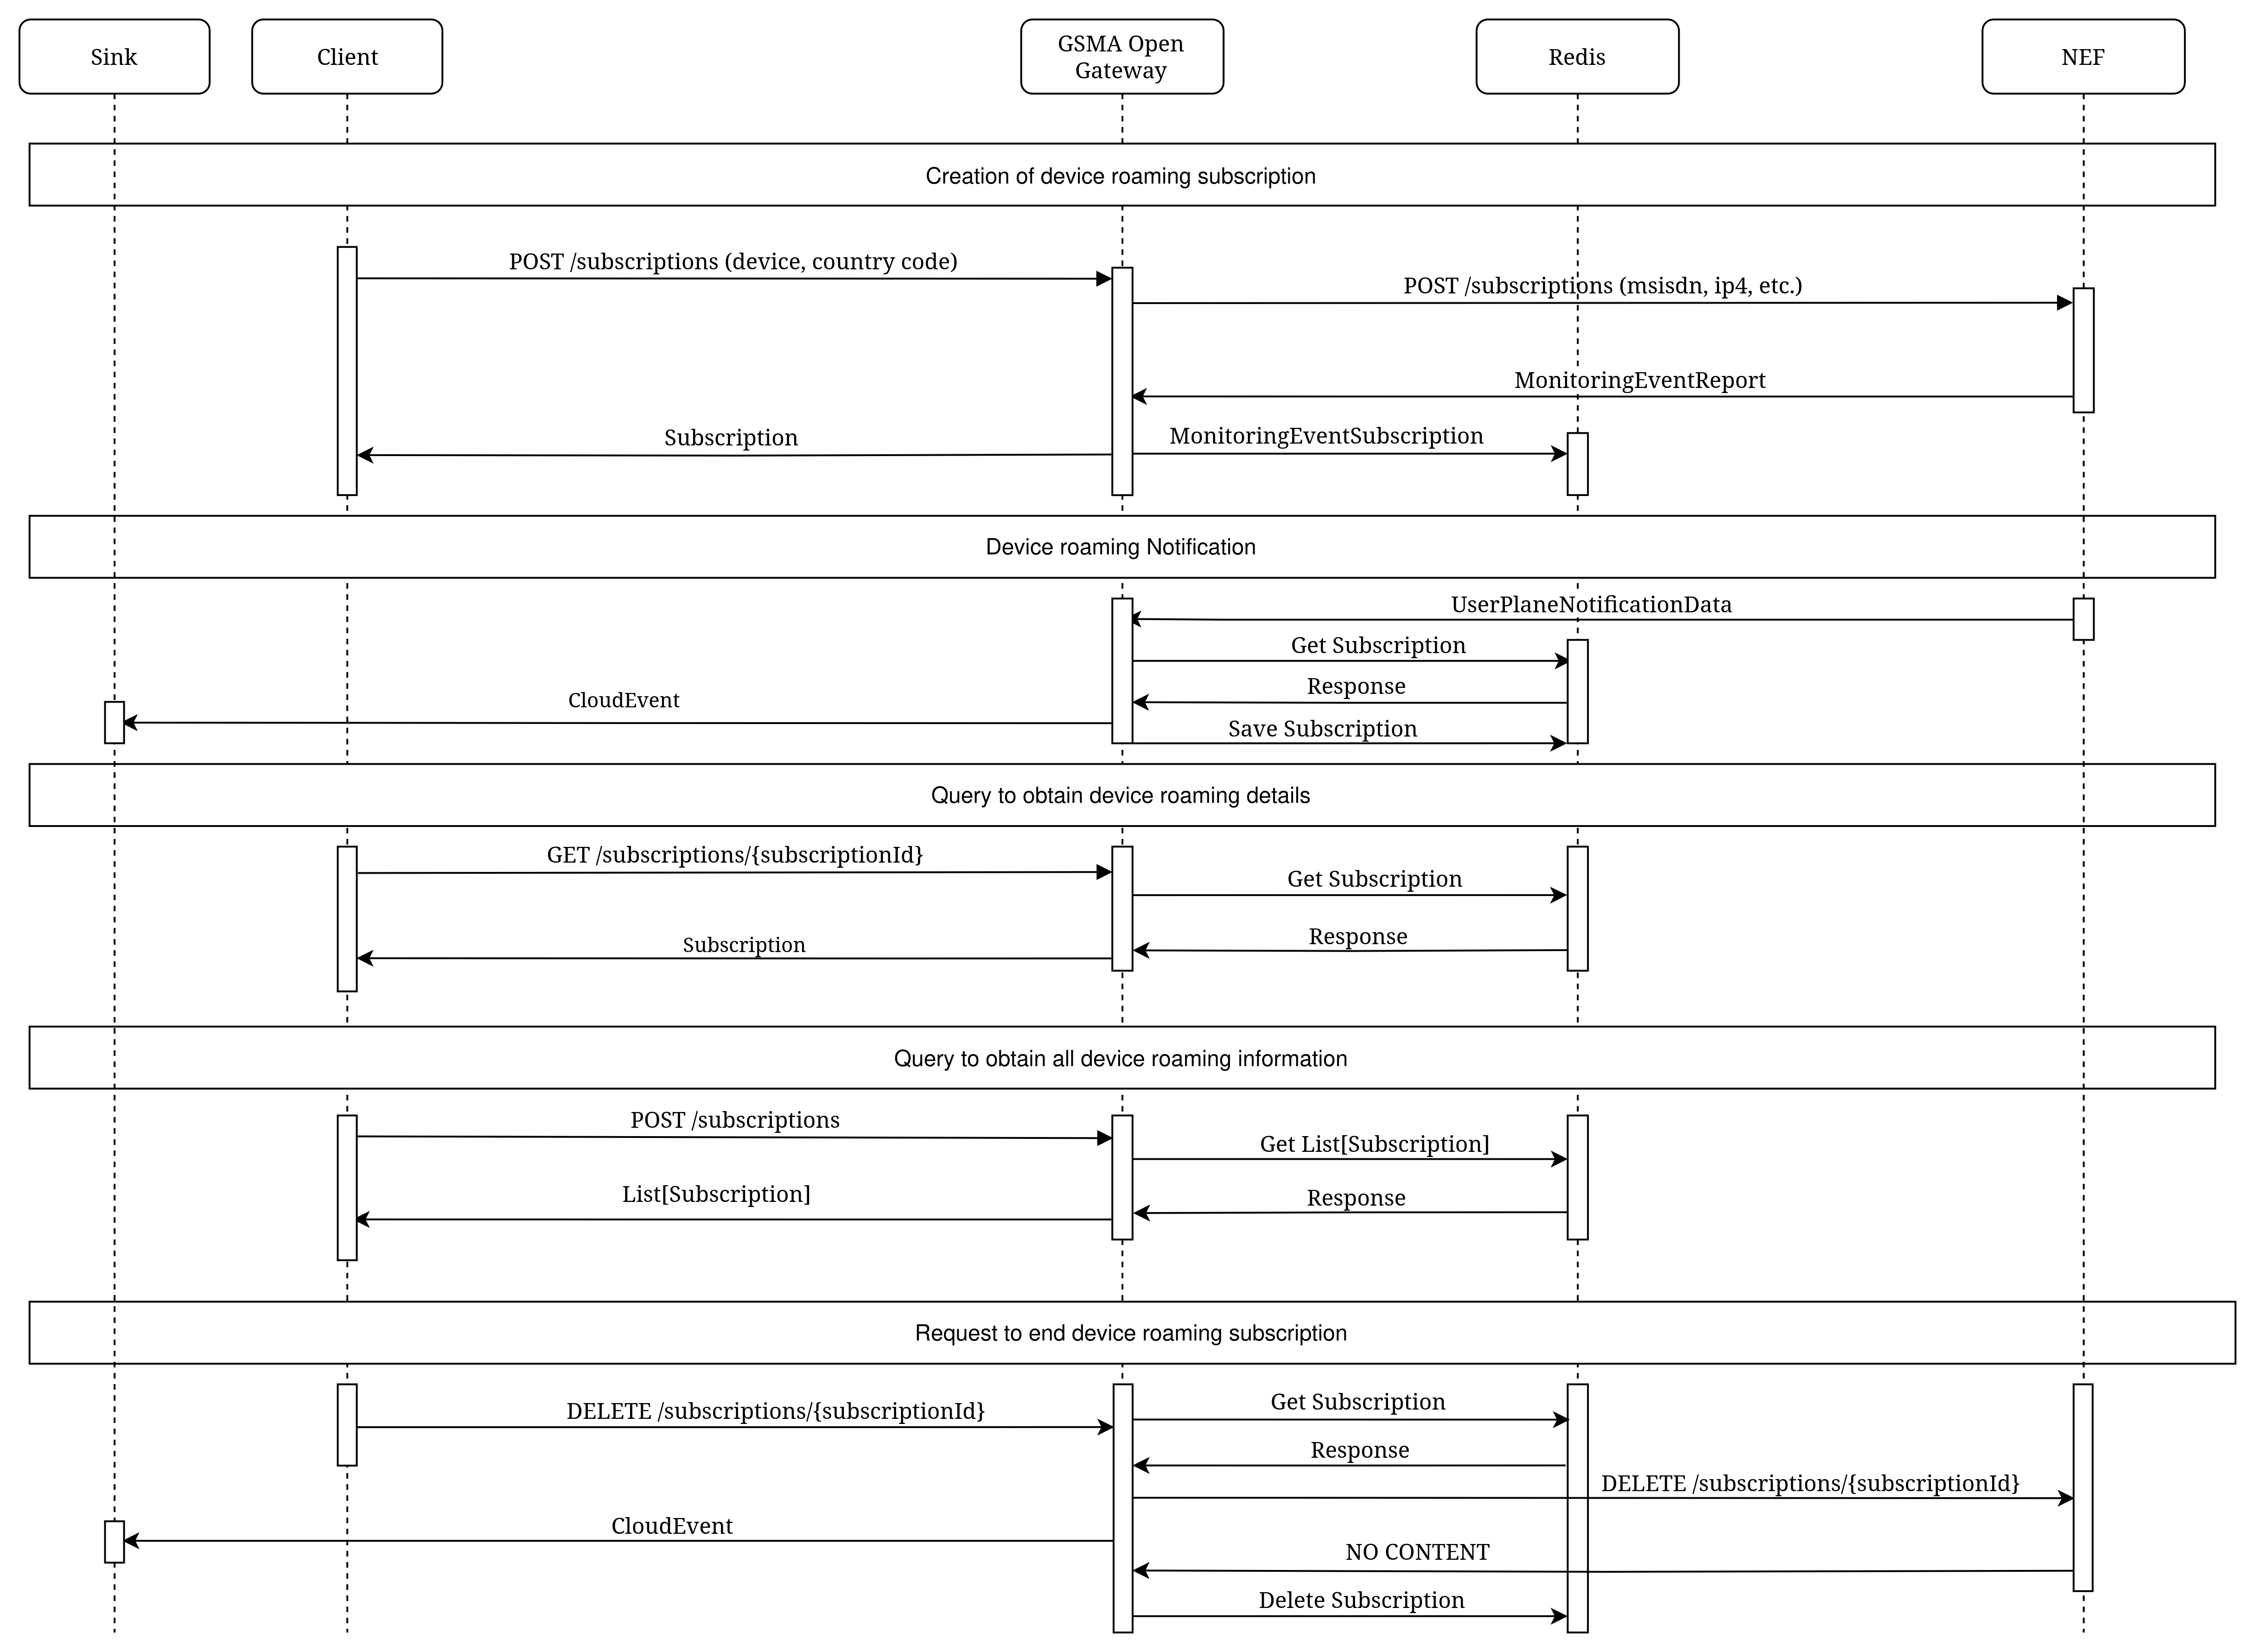
\includegraphics[width=15cm]{figs/roaming_sub_sequence_diagram.png}
	}
	\caption{Device Roaming Status Subscription Sequence Diagram}
\end{figure}
